\newpage{\ } 
\thispagestyle{empty} 

\chapter{Materiales y Metodolog\'ia}
\lhead{Capítulo 4. \emph{Materiales y Metodolog\'ia}} % This is for the header on each page - perhaps a shortened title
En este cap\'itulo se describir\'an los materiales a utilizar en la elaboraci\'on de la metodolog\'ia, as\'i como tambi\'en aquellos a utilizar en las diversas pruebas y validaciones. Adem\'as se presentan las diversas características de las imágenes satelitales a ser empleados en el estudio. La metodolog\'ia nos presenta los diferentes procesos o m\'odulos necesarios para la estimaci\'on de p\'erdida de carbono.
\section{Materiales}
Un grupo de im\'agenes fueron utilizadas para los diferentes estudios y procedimientos de la metodologia, tales como:
\begin{itemize}
	\item Im\'agenes satelitales Landsat.
	\item Im\'agenes Campos Continuos de Vegetación (VCF).
	\item Im\'agen Mapa global de carbono - Paraguay.
	\item Paraguay Forest Change Product.
\end{itemize}
En el procesamiento e implementaci\'on de algoritmos fueron utilizados dos aplicaciones:
\begin{itemize}
	\item GRASS.
	\item Quantum GIS.
\end{itemize}
A continuaci\'on se hablaran con mayor detalle de los elementos citados.
\subsection{Im\'agenes}
En este apartado se pretende brindar las diferentes caracter\'isticas que presentan cada tipo de imagen utilizada en este trabajo..
\subsubsection{Landsat}\label{sec:landsat}
Landsat representa la colecci\'on m\'as larga y continua en el mundo de im\'agenes satelitales con resoluciones moderadas \cite{landsatNasa}. Cuatro d\'ecadas de im\'agenes proporciona un recurso \'unico para personas que trabajan en la agricultura, geolog\'ia, silvicultura, ordenaci\'on territorial, educaci\'on, cartograf\'ia e investigaci\'on del cambio global, como tambi\'en en respuesta de emergencias y operaciones de socorro.\\~\\
Las im\'agenes est\'an disponibles desde 1972 generados por una serie de 6 sat\'elites Landsat. Estos sat\'elites han sido un componente importante del Programa de Observaci\'on de la tierra perteneciente a la NASA, con tres sensores primarios evolucionando a lo largo de treinta años: MSS (Multi-spectral Scanner), TM (Thematic Mapper), y ETM+ (Enhanced Thematic Mapper Plus). 
El 11 de febrero del 2013 fue lanzado el Lansadt 8 correspondiendo al futuro de los sat\'elites Landsat con dos nuevo sensores, Operational Land Imager (OLI) y el Thermal Infrared Sensor (TIRS). La Tabla \ref{t:landsattipos} nos muestra las diferentes resoluciones de los sensores Landsat.

\begin{table}[htb!]
	\centering
	\begin{tabular}{|c|c|c|c|c|c|}
		\hline
		\multirow{2}{*}{\textbf{Landsat}} & \multicolumn{5}{c|}{\textbf{Resoluciones}}                                                             \\ \cline{2-6} 
		& \textbf{Espacial} & \textbf{Espectral} & \textbf{Radiom\'etrica} & \textbf{Temporal} & \textbf{Sensor} \\ \hline
		1                                 & 79x79 m2          & 5 bandas           & 6 bits                  & 18 dias           & MSS             \\ \hline
		2                                 & 79x79 m2          & 5 bandas           & 6 bits                  & 18 dias           & MSS             \\ \hline
		3                                 & 79x79 m2          & 5 bandas           & 6 bits                  & 18 dias           & MSS             \\ \hline
		4                                 & 30x30 m2          & 7 bandas           & 8 bits                  & 16 dias           & TM              \\ \hline
		5                                 & 30x30 m2          & 7 bandas           & 8 bits                  & 16 dias           & TM              \\ \hline
		6                                 & 30x30 m2          & 8 bandas           & 8 bits                  & 16 dias           & ETM+            \\ \hline
		7                                 & 30x30 m2          & 8 bandas           & 8 bits                  & 16 dias           & ETM+            \\ \hline
		8                                 & 30x30 m2          & 9 bandas           & 12 bits                 & 16 dias           & OLI/TIRS        \\ \hline
	\end{tabular}
	\caption{Resoluciones de los sat\'elites Landsat.}
		\label{t:landsattipos}
\end{table}
El Sistema de Referencia Mundial Landsat-2 (WRS-2: Landsat Worldwide Reference System-2) provee un esquema de indexaci\'on para el patr\'on de repetici\'on de la trayectoria orbital terrestre seguida por las plataformas espaciales Landsat 4, 5 y 7 sobre los 16 d\'ias de su repetitivo ciclo orbital \cite{els2015refere}. El original WRS (WRS-1) fue dise\~{n}ado para las misiones Landsat 1, 2, y 3, las cuales se movieron en una \'orbita m\'as alta. El actual WRS-2 fue dise\~{n}ado para la \'orbita a 705 Km usada para las \'ultimas misiones. En la Figura \ref{fig:wrs2Image} podemos observar los \'indices (Path y Row) en el momento de la obtenci\'on de una imagen satelital Landsat para una zona.

\begin{figure}[H]
	\centering
	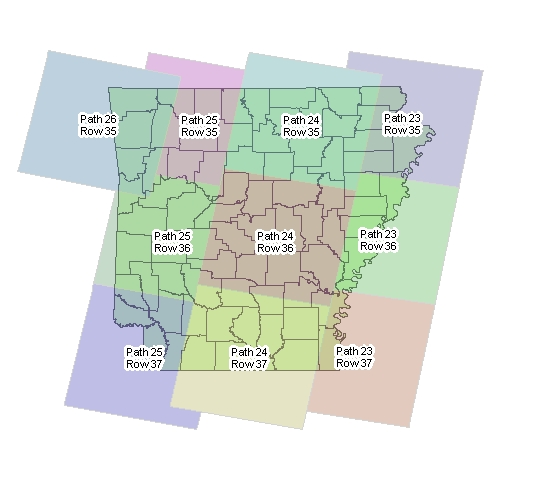
\includegraphics[width=0.8	\textwidth]{./Figures/cap4/wrs2_22.jpg}
	\caption{Ejemplo WRS-2 Path/Row}
	\label{fig:wrs2Image}
\end{figure}

El Servicio Geol\'ogico de los Estados Unidos (USGS) es una agencia cient\'ifica de los Estados Unidos, el cual proveen un producto llamado L1T (Level 1 Terrain Corrected) que implica las im\'agenes Landsat con datos pre-procesados para una correcci\'on radiom\'etrica sistem\'atica y correcci\'on geom\'etrica mediante la incorporaci\'on de puntos de control en tierra. Estos productos est\'an en la Web de forma gratuita \cite{landsatNasa}.


\subsubsection{Campos Continuos de Vegetación (VCF)}\label{sec:vcf}
Las im\'agenes VCF contienen estimaciones proporcionales para los tipos de cobertura vegetal: vegetaci\'on le\~{n}osa, vegetaci\'on herb\'acea y suelo desnudo. El producto se deriva de las siete bandas del sensor MODerate-resolution Imaging Spectroradiometer (MODIS) a bordo del sat\'elite Terra, perteneciente a la NASA. El esquema de clasificaci\'on continuo del VCF puede representar \'areas terrestres heterog\'eneas mejor que los esquemas tradicionales de clasificaci\'on discreta. Los sistemas de clasificaci\'on tradicionales indican donde se concentran los tipos de cobertura del suelo. El VCF posee un resoluci\'on espacial de 250x250 metros cuadrados y la colecci\'on de im\'agenes se encuentra disponible gratuitamente en la Web \cite{gl2015Uni}.
La Figura \ref{fig:vcfImage} nos presenta un imagen, con diferentes tonalidades de color, para los porcentajes de vegetaci\'on y los niveles digitales del agua como pixeles nulos.
\begin{figure}[H]
	\centering
	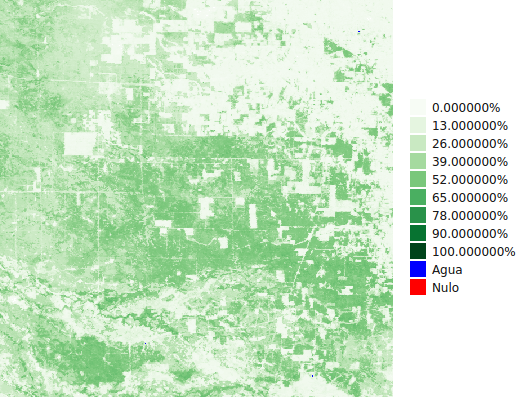
\includegraphics[width=0.8	\textwidth]{./Figures/cap4/vcf_image.png}
	\caption{Imagen VCF con diferentes tonalidades de color de acuerdo al porcentaje de vegetaci\'on.}
	\label{fig:vcfImage}
\end{figure}
\subsubsection{Mapa global de carbono - Paraguay}\label{sec:saatchiMapa}
El mapa global de carbono \cite{saatchi2011benchmark} nos provee la densidad de carbono, expresada en toneladas de carbono por hect\'area, del \'area ocupada por un pixel. El mapa fue elaborado para la d\'ecada de los 2000. En la actualidad existen diferentes mapas de carbono a nivel mundial \cite{saatchi2011benchmark}. La Figura \ref{fig:saatchi} representa el mapa global de carbono disponible para el Paraguay.
\begin{figure}[H]
	\centering
	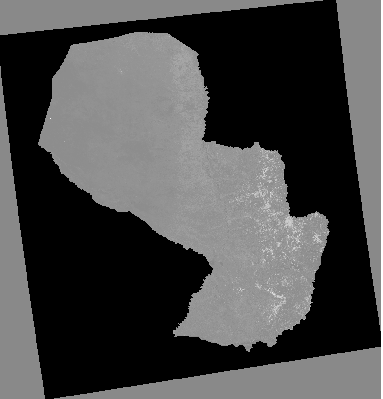
\includegraphics[width=0.8	\textwidth]{./Figures/cap5/saatchi.png}
	\caption{Mapa Global de Carbono - Paraguay}
	\label{fig:saatchi}
\end{figure}


\subsubsection{Paraguay Forest Change Product}\label{sec:fcc}
El Paraguay Forest Change Product (PFCP) muestra donde ocurri\'o la deforestaci\'on en Paraguay durante 1990-2000. El PFCP fue elaborado a partir de las im\'agenes Landsat TM y ETM+, identificando seis clases; bosque atl\'antico, Chaco bosques, el agua, no forestales y la deforestaci\'on. El producto puede ser utilizado para determinar procesos y patrones de cambio en la cubierta forestal. En la Figura \ref{fig:fcc} se puede observar el PFCP (disponible gratuitamente \cite{gl2015Uni}). En la Tabla \ref{t:pfcptab} se describe la representaci\'on de cada nivel digital en dicha imagen. .
\begin{table}[htbp]\centering
\begin{tabular}{|c|c|c|}
	\hline \textbf{Valor digital} &\textbf{ Representaci\'on} & \textbf{Color sugerido} \\ 
	\hline 1 & Bosque Atl\'antico & Verde \\ 
	\hline 2 & Bosque Chaque\~{n}o & Verde Claro \\ 
	\hline 3 & No Bosque & Agua \\ 
	\hline 4 & Agua & Azul \\ 
	\hline 5 & P\'erdida Bosque Atl\'antico & Rojo \\ 
	\hline 6 & P\'erdida Bosque Chaque\~{n}o & Purpura Claro \\ 
	\hline 
\end{tabular} 
\caption{Representaci\'on del valor digital en la imagen PFCP.}
\label{t:pfcptab}
\end{table}

\begin{figure}[H]
	\centering
	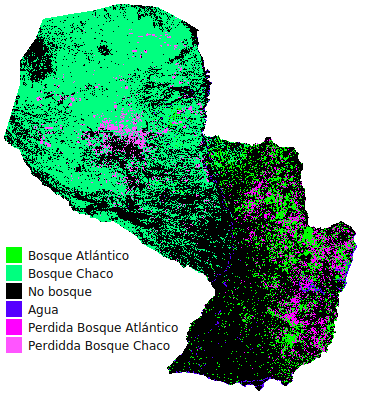
\includegraphics[width=0.7	\textwidth]{./Figures/cap4/fcc_paraguay.png}
	\caption{Paraguay Forest Change Product}
	\label{fig:fcc}
\end{figure}



\subsection{Aplicaciones}
Sistemas de informaci\'on geogr\'afica fueron utilizados para la manipulaci\'on de im\'agenes satelitales, como tambi\'en para dise\~{n}ar e implementar los algoritmos utilizados en la metodolog\'ia propuesta. A continuaci\'on se describen las aplicaciones utilizadas.

\begin{itemize}
	\item \textbf{GRASS: }es un software SIG  bajo licencia GPL (software libre) \cite{osgeoGrass}. El software soporta informaci\'on tanto raster como vectorial y posee herramientas de procesado digital de im\'agenes. Esta disponibles principalmente para plataformas Linux.
	\item \textbf{Quantum GIS: }es un SIG de c\'odigo libre para plataformas GNU/Linux, Unix, Mac OS, Microsoft Windows y Android. La principal diferencia con el GRASS es la interfaz amigable con que cuenta y la facilidad de integraci\'on con nuevas funciones espaciales desarrollados por los usuarios \cite{qgisSIG}.
\end{itemize}

\section{Metodolog\'ia}
Los datos de entrada son las im\'agenes Landsat pre-procesadas (correcciones geom\'etricas y radiom\'etricas) de manera a disminuir los errores de localizaci\'on e intensidad de los niveles digitales causados por distintos factores (secci\'on \ref{sec:correcionesImages}).  
Las im\'agenes Landsat 8 no deben ser mezcladas con im\'agenes de otro sensor del mismo sat\'elite, ya que esta posee una resoluci\'on radiom\'etrica de 16 bits y las dem\'as son capturadas a 8 bits. Las bandas utilizadas corresponde a la infrarroja cercana y roja.\\~\\
En la Figura \ref{fig:metodologiapc} podemos observar que a partir de las banda infrarroja cercana y roja ($ f_{t}(x,y,IRc);f_{t}(x,y,R) $, $ f_{t_{*}}(x,y,IRc);f_{t_{*}}(x,y,R) $) de una secuencia multitemporal, donde $ t < t_{*} $, es posible obtener una mascara de perdida forestal $ MPF $ y su cuantificaci\'on ($ CCP $) en toneladas de carbono perdidos ($ ton $ $ C $) una vez pasado por los procesos de detecci\'on de cambio forestal y estimaci\'on de p\'erdida de carbono Forestal.
\begin{figure}[H]
	\centering
	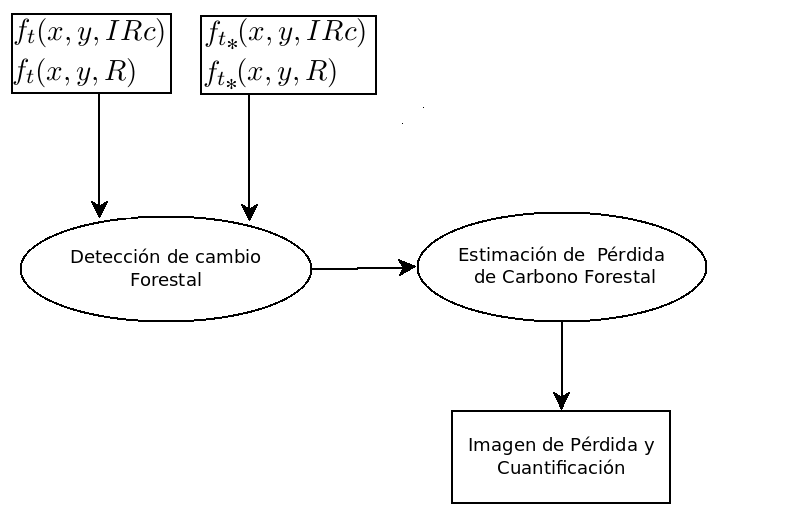
\includegraphics[width=0.8	\textwidth]{./Figures/cap4/metodologiaCarbono_3.png}
	\caption{Diagrama de flujo. Metodolog\'ia propuesta}
	\label{fig:metodologiapc}
\end{figure}

\subsection{Detecci\'on de cambio Forestal}
La detecci\'on de cambio cumple un papel fundamental en la metodolog\'ia ya que nos permite categorizar el cambio en la secuencia temporal estudiada. Este proceso presenta una metodolog\'ia automatizada a trav\'es del calculo de par\'ametros estad\'isticos extra\'ido de las im\'agenes satelitales y el uso de variables determinadas en un previo an\'alisis del comportamiento espectral observados en la cobertura vegetal de prueba.

\subsubsection{Detecci\'on de cambio}
En este proceso se detecta el cambio entre dos tiempos de im\'agenes satelitales. El resultado esperado constituye una mascara de perdida ($ MP $) entre las series temporales de im\'agenes comparadas. 
\paragraph{Comparaci\'on Multitemporal}\mbox{}\\\mbox{}\\
El siguiente paso despu\'es de haber equiparado radiom\'etricamente (secci\'on \ref{sec:capNormalizacion}) las im\'agenes consiste en la comparaci\'on multitemporal, permitiendo obtener un indice de cambio (variable cuantitativa) en cada pixel resultante. El m\'etodo de diferencia de im\'agenes es utilizada debido a que el m\'etodo Ratio no se ajusta a una distribuci\'on normal, se asume que el cambio es reducido y por ende est\'an ubicados hacia los extremos del histograma de la imagen con los \'indices de cambio $ I_{c} $, condici\'on clave para la umbralizaci\'on estad\'istica. La comparaci\'on es realizado sobre la imagen con los NDVI de cada serie temporal a modo a resaltar la vegetaci\'on y simplificar la cantidad de bandas utilizadas, observando a su vez que los datos estables ser\'an pr\'oximos a $ 0 $ gracias a la semejanza existente entre los pixeles. 
\paragraph{Umbral estad\'istico} \label{sec:umbralEstadistico2}\mbox{}\\\mbox{}\\
Los criterios de decisi\'on propuesto en la secci\'on \ref{sec:discriminacion} asignan valores de cambio/no cambio en funci\'on a un umbral. Estos criterios permiten convertir los indices de cambios a valores cualitativos que representan una m\'ascara de cambio ($ MC $). El m\'etodo basados en par\'ametros estad\'isticos es escogido por su sencillez y coherencia con el m\'etodo de comparaci\'on multitemporal aplicada. Los niveles digitales de $ MC $ est\'an definidos por la siguiente expresi\'on:
\begin{equation}\label{ec:umbMetodo}
MC(x,y) = \begin{cases}
1 & \text{si se cumple que } \mu_{I_{c}} - n \times \sigma_{I_{c}} < I_{c}(x,y) < \mu_{I_{c}} + n \times \sigma_{I_{c}}\\
0 & \text{cualquier otro caso}  
\end{cases}
\end{equation}
En la Figura \ref{fig:umbrales} se puede observar una linea roja y verde, que determinan los limites para los cuales los \'indices no son considerados pixeles de cambio (pixeles que no variaron con respecto al tiempo). La variable de fiabilidad $ n $ es elegida en base a la probabilidad de cambio deseado para la detecci\'on (secci\'on \ref{sec:discriminacion}).
	\begin{figure}[H]
		\centering
		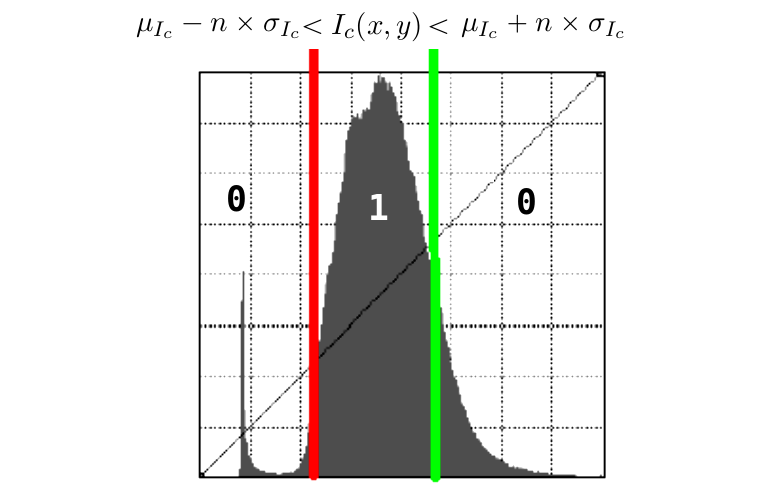
\includegraphics[width=0.8	\textwidth]{./Figures/cap4/umbrales_3.png}
		\caption{Umbrales que binarizan los indices de cambios $ I_{c} $.}
		\label{fig:umbrales}
	\end{figure}
Los pixeles que sufrieron perdida estar\'an definidos por una m\'ascara $ MP $ con las siguiente expresi\'on:
\begin{equation}\label{ec:umbMetodoMP}
MP(x,y) = \begin{cases}
1 & \text{si se cumple que } I_{c}(x,y) < \mu_{I_{c}} - n \times \sigma_{I_{c}} \\
0 & \text{cualquier otro caso}  
\end{cases}
\end{equation}
\paragraph{Iteraci\'on}\label{subsec:iteracion}\mbox{}\\\mbox{}\\
 Si dos im\'agenes se consideran semejantes, los cambios producidos en el terreno afectan a la radiometr\'ia registrada en las im\'agenes, y por tanto, en los par\'ametros estad\'isticos que las definen.\\~\\
En la normalizaci\'on radiom\'etrica los cambios introducen ruido \cite{martinez2013normalizacion}, ya que el proceso busca que los pixeles de una banda de im\'agenes satelitales en diferentes tiempos sean semejantes y el cambio estar\'ia influyendo en la correlaci\'on entre los pixeles que verdaderamente no sufrieron cambio. Si el \'area de todos los pixeles con cambio es mayor, la influencia en la normalizaci\'on ser\'a mayor y por ende afectara la precisi\'on en la detecci\'on de cambios. En vista al problema, mediante una normalizaci\'on radiom\'etrica iterativa se pretende minimizar dicha influencia, donde los par\'ametros estad\'isticos ($ \mu,\sigma $) utilizados constituyen los pixeles sin cambios.\\~\\	
La Figura \ref{fig:deteccionCambio} nos presenta el ciclo de procedimientos para la detecci\'on de cambio, donde a partir de la secuencia de im\'agenes satelitales en las bandas infrarroja cercana y roja ($ f_{t}(x,y,IRc);f_{t}(x,y,R), f_{t_{*}}(x,y,IRc);f_{t*}(x,y,R) $) son calculados los par\'ametros estad\'isticos ($ \mu_{i,t};\sigma_{i,t}, \mu_{i,t_{*}};\sigma_{i,t_{*}} $) para las im\'agenes. Esos par\'ametros son utilizados para normalizar radiom\'etricamente las bandas del tiempo $ t_{*} $, en semejanza a las bandas de la imagen satelital del tiempo $ t $, as\'i determinar la imagen con los \'indices de cambios ($ I_{c} $) una vez calculados los NDVI ($ ndvi_{f_{t}},ndvi_{f_{t_{*}}} $). La m\'ascara de cambio ($ MC $) es el resultado de pasar por los umbrales estad\'isticos (secci\'on \ref{sec:umbralEstadistico2}). La iteraci\'on ($ iter $) continua si la media del $ I_{c} $ actual es de magnitud similar a la registrada en la anterior. Se define la función l\'ogica $ continuar $:
  \begin{equation}\label{ec:continuar}
  continuar(\mu_{I_{c}^{iter}},\mu_{I_{c}^{iter-1}}) = \begin{cases}
  falso & \text{si se cumple que } \mu_{I_{c}^{iter}} - \mu_{I_{c}^{iter-1}} \leq \epsilon \\
  verdadero & \text{en cualquier otro caso }
  \end{cases}
  \end{equation}
  \nomenclature[58]{$ \epsilon $}{Error de cambio.}
  Siendo $ \epsilon $ un error de aproximaci\'on. Si el proceso de iteraci\'on debe continuar, el c\'alculo  de los par\'ametros estad\'isticos debe realizarse seg\'un el Algoritmo \ref{alg:parametros}. Cada valor de pixel, de las bandas en cada imagen satelital, es utilizado en el c\'alculo si no representa un cambio en la m\'ascara de cambio $ MC $.
  \begin{algorithm}[H]
  	\caption{Funci\'on que calcula los par\'ametros estad\'isticos.}
  	\label{alg:parametros}
  	\begin{algorithmic}[1]
  		\Statex
  		\Function {parametros}{$f_{t}(x,y,R),f_{t}(x,y,IRc),MC$}
		\State $sumR =0$ \Comment{Variable auxiliar sumatoria}
		\State $sumIRc =0 $ \Comment{Variable auxiliar sumatoria}
		\State $nT =0 $ \Comment{N\'umero de pixeles sin cambio}
		\Statex
		\For {$x \gets 0, fil$}
			\For {$y \gets 0, col$}
%															\algstore{myalg2}
%														\end{algorithmic}
%													\end{algorithm}
													
%													\begin{algorithm}                     
%														\begin{algorithmic} [1]                   % enter the algorithmic environment
%															\algrestore{myalg2}
				\If{$MC(x,y)=1$}
					\State $sumR=sumR+f_{t}(x,y,R)$
					\State $sumIRc=sumIRc+f_{t}(x,y,IRc)$
					\State $nT=nT++$
				\EndIf
			\EndFor
		\EndFor
	\Statex
		\State $ \mu_{R,t}= sumR/nT$
		\State $ \mu_{IRc,t}= sumIRc/nT$
		\State $ sumR=0$
		\State $ sumIRc=0$
		\Statex
		\For {$x \gets 0, fil$}
			\For {$y \gets 0, col$}
				\If{$MC(x,y)=1$}
					\State $sumR=sumR+(f_{t}(x,y,R)-\mu_{R,t})^{2}$
					\State $sumIRc=sumIRc+(f_{t}(x,y,IRc)-\mu_{IRc,t})^{2}$
				\EndIf
			\EndFor
		\EndFor
		\Statex
		\State $\sigma_{R,t}=\sqrt{\dfrac{1}{nT-1} \times sumR}$
		\State $\sigma_{IRc,t}=\sqrt{\dfrac{1}{nT-1} \times sumIRc}$
  		\Statex
  		\Return $[\mu_{R,t},\mu_{IRc,t},\sigma_{R,t},\sigma_{IRc,t}]$
  		\EndFunction
  	\end{algorithmic}
  \end{algorithm}
El proceso de iteraci\'on finaliza retornando una un m\'ascara de perdida $ MP $ seg\'un la ecuaci\'on \ref{ec:umbMetodoMP}.\\~\\
\begin{figure}[H]
	\centering
	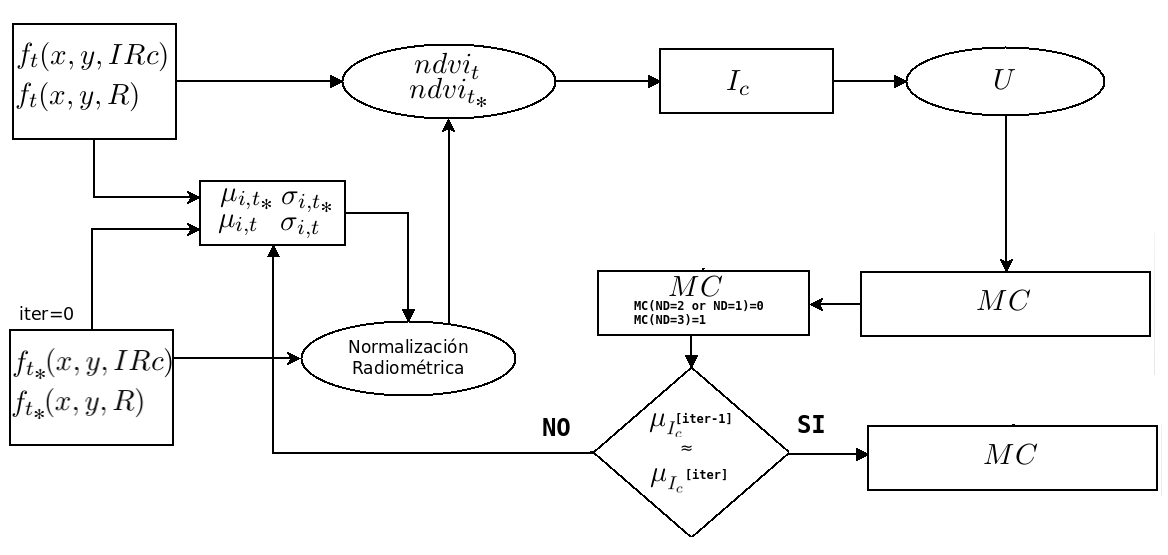
\includegraphics[width=1.0 \textwidth]{./Figures/cap4/deteccionCambio_4.png}
	\caption{Diagrama de flujo. Detecci\'on de Cambio.}
	\label{fig:deteccionCambio}
\end{figure}

En la Figura \ref{fig:iteracionRadiometrica} podemos observar que a partir de la mascara de cambio obtenido en la primera iteraci\'on, los par\'ametros estad\'isticos para la iteraci\'on 2, en la normalizaci\'on iterativa, son realizados sobre los pixeles que no detectaron cambios. 
\begin{figure}[H]
	\centering
	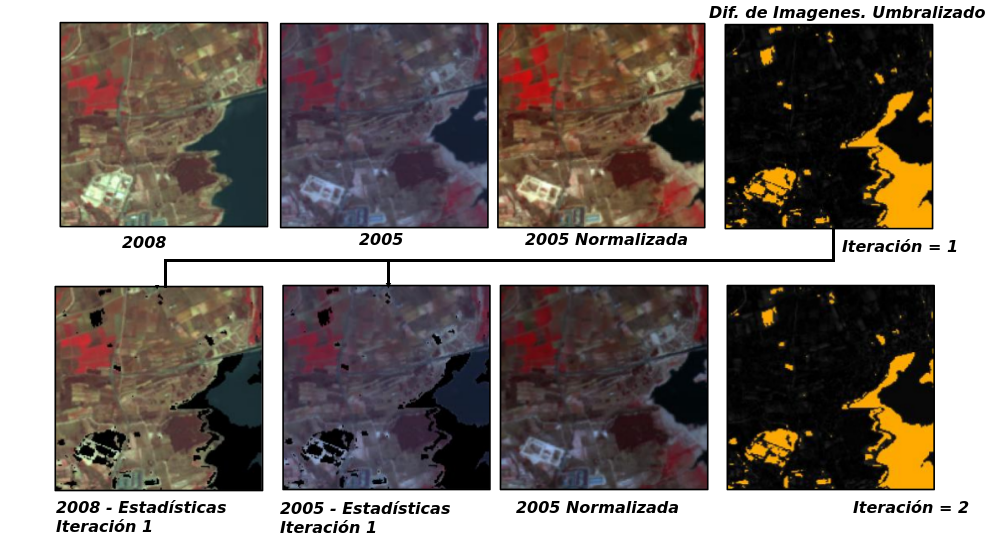
\includegraphics[width=1.0	\textwidth, height=0.5 \textheight]{./Figures/cap4/iteracionUmbra.png}
	\caption{Mascaras de cambio, iteraci\'on de la normalizaci\'on radiom\'etrica.}
	\label{fig:iteracionRadiometrica}
\end{figure}


\subsubsection{Discriminaci\'on Forestal}\label{sec:discrForestalMet}
Las im\'agenes procesadas son aquellas obtenidas en la ultima normalizaci\'on radiom\'etrica, generada por el proceso iterativo y la imagen base para la semejanza en ese proceso. En este procedimiento se busca generar una mascara de vegetaci\'on (MV) de la secuencia temporal.
\paragraph{NDVI}\mbox{}\\\mbox{}\\
El NDVI es calculado para ambas fechas pertenecientes a la secuencia multitemporal evaluada ($ndvi_{f_{t}},ndvi_{f_{t_{*}}}  $). El calculo es hecho teniendo como entradas las bandas infrarroja cercana y roja, donde el vigor vegetal de cada p\'ixel sera determinado por la ecuaci\'on \ref{e:ndvi}. 
\paragraph{Umbral de Vegetaci\'on}\label{sec:uvegetacion}\mbox{}\\\mbox{}\\
El umbral que binariza la vegetaci\'on es determinado a partir de una constante calculada por un previo an\'alisis del comportamiento espectral de la cobertura vegetal y las im\'agenes de NDVI, retornando una imagen binarizada $ ndvi_{f_{t}}^{B} $ dado un $ ndvi_{f_{t}} $. Dicha variable corresponde a la desviaci\'on observada $(\sigma_{c}) $ en la intersecci\'on de puntos de muestreo aleatorios entre im\'agenes VCF y Landsat (secci\'on \ref{subsec:umbralVegetacion}). La ecuaci\'on que determina a $ ndvi_{f_{t}}^{B} $ tiene la siguiente expresi\'on:
  \begin{equation}\label{ec:umbVegetacion}
  ndvi_{f_{t}}^{B}(x,y) = \begin{cases}
  1 & \text{si se cumple que } ndvi_{f_{t}}(x,y) > \mu_{ndvi_{f_{t}}}-n \times \sigma_{c}  \\
  0 & \text{en cualquier otro caso }
  \end{cases}
  \end{equation}
\nomenclature[58]{$ \sigma_{c} $}{Desviaci\'on determinada como constante para la umbralizaci\'on de la cobertura vegetal.}
Donde $ \mu_{ndvi_{f_{t}}} $ representa la media de la imagen $ ndvi_{f_{t}} $ y $ n $ el coeficiente de fiabilidad. En la Figura \ref{fig:ndviUmbral} podemos observar que el umbral del NDVI (linea roja) se situ\'a por debajo de la media (linea fucsia) permiti\'endonos discriminar los pixeles que representan vegetaci\'on/no vegetaci\'on.
\begin{figure}[H]
	\centering
	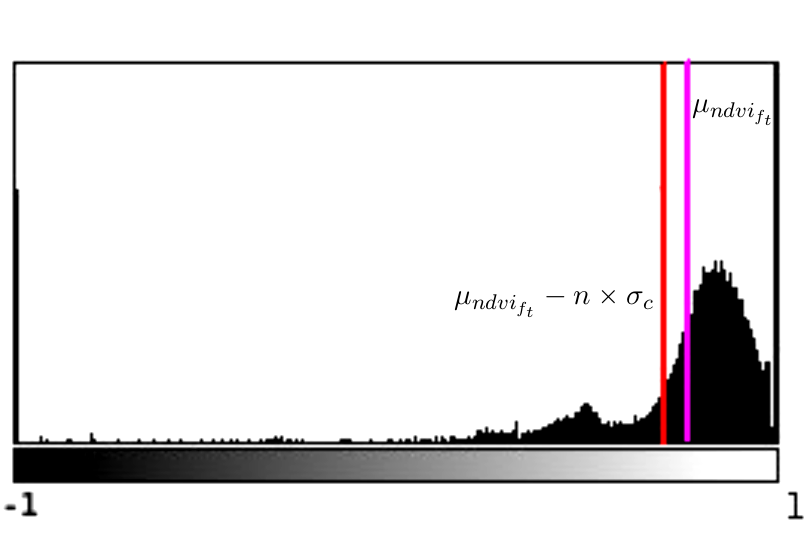
\includegraphics[width=0.8	\textwidth]{./Figures/cap4/ndviUmbral_2.png}
	\caption{Umbral utilizado y la media en el histograma de la imagen con NDVI.}
	\label{fig:ndviUmbral}
\end{figure}

\paragraph{Intersecci\'on \'area boscosa }\mbox{}\\\mbox{}\\
El procedimiento que sigue una vez obtenido los NDVI de las dos fechas es determinar los pixeles que ser\'an evaluados para detectar el cambio, por ello aplicamos una simple operaci\'on de uni\'on ($ ndvi_{f_{t}}^{B} $ OR $ ndvi_{f_{t_{*}}}^{B}$) que generara una mascara de vegetaci\'on $ MV $ correspondiente a los dos tiempos. La Figura \ref{fig:discrimForestal} refleja los pasos realizados para obtener una mascara de vegetaci\'on.
\begin{figure}[H]
	\centering
	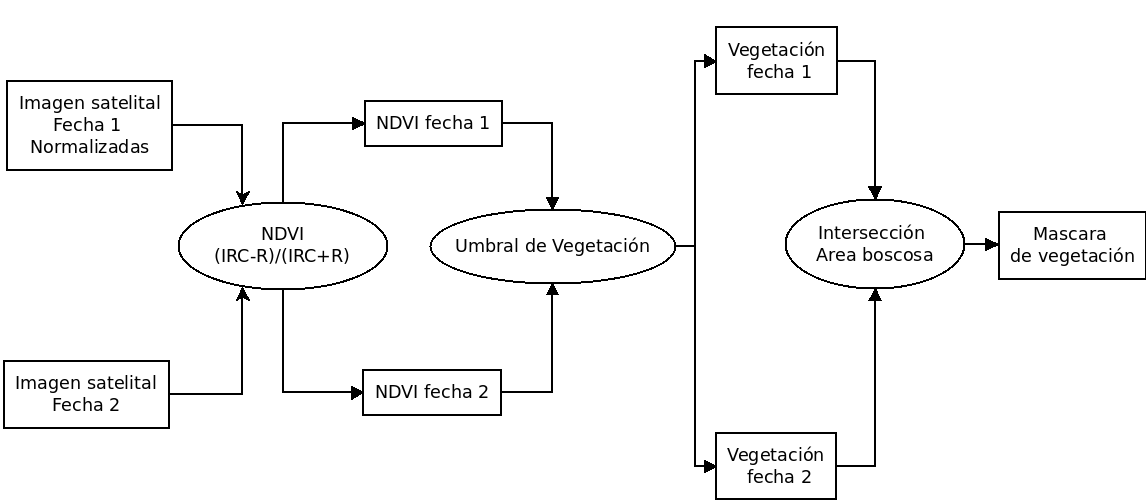
\includegraphics[width=1.0	\textwidth]{./Figures/cap4/discriminacionForestal_2.png}
	\caption{Diagrama de flujo. Discriminaci\'on Forestal.}
	\label{fig:discrimForestal}
\end{figure}


\subsubsection{Mascara de P\'erdida Forestal}
El proceso consiste en la intersecci\'on entre la mascaras de vegetaci\'on y cambio. En la intersecci\'on solo son considerados los cambios correspondiente a p\'erdidas  $ MP $, debido a que se pretende generar una imagen binaria $ MPF $ que represente la perdida forestal en un pixel.\\~\\
La imagen $ MPF $ probablemente tendr\'a errores que son inherentes a los procesos utilizados para su creación \cite{lovell2001filtering}. Estos errores lo consideramos como ruidos en la imagen $ MPF $. El filtro de mediana \cite{gonzalez2002woods} reducir\'a el porcentaje de falsas alarmas en la imagen $ MPF $ eliminando los ruidos generados.
En la Figura \ref{fig:intersPerdida} podemos observar el flujo de tareas para la obtenci\'on de la mascara que representa la perdida forestal en dos tiempos .
\begin{figure}[H]
	\centering
	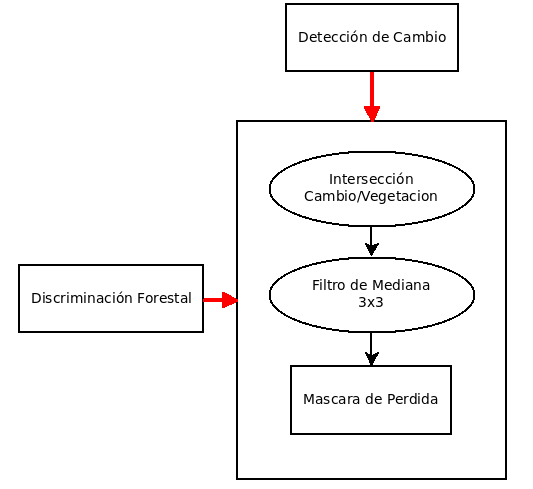
\includegraphics[width=0.6	\textwidth]{./Figures/cap4/interseccionPerdida.png}
	\caption{Diagrama de procedimientos para la obtenci\'on de la m\'ascara de perdida forestal.}
	\label{fig:intersPerdida}
\end{figure}

\subsection{Estimaci\'on de p\'erdida de carbono forestal}
El procedimiento final en la metodolog\'ia consiste en estimar el carbono perdido o no secuestrados dentro del tiempo transcurrido entre las im\'agenes satelitales. El producto constituye la mascara de perdida forestal ($ MPF $) junto con la cuantificaci\'on ($ CCP $) en toneladas de carbono obtenida a trav\'es de una ecuaci\'on de regresi\'on lineal. La ecuaci\'on de regresi\'on fue generada por medio del mapa global de carbono (variable dependiente) \cite{saatchi2011benchmark} y el NDVI (variable independiente) determinadas por las im\'agenes Landsat en un an\'alisis previo (m\'as detalles en la secci\'on \ref{subsec:estimacionCarbono}). La regresi\'on fue evaluada a trav\'es del coeficiente de determinaci\'on $ r^{2} $. En la Tabla \ref{t:coefDeter} se presenta el tipo de relaci\'on del coeficiente de determinaci\'on \cite{kris2014estimacionCorr}.
\nomenclature[59]{$ r^{2}$}{Coeficiente de determinaci\'on para una regresi\'on.}
\begin{table}[H]
	\centering
	\begin{tabular}{|l|l|}
		\hline
		\textbf{Valor} & \textbf{Significado} \\ \hline
		0,0            & Ninguna Relaci\'on     \\ \hline
		0,25           & Relaci\'on baja        \\ \hline
		0,50           & Relaci\'on Moderada    \\ \hline
		0,75           & Relaci\'on Buena       \\ \hline
		1,00           & Relaci\'on perfecta    \\ \hline
	\end{tabular}
	\caption{Rangos del coeficiente de determinaci\'on.}
	\label{t:coefDeter}
\end{table}

Sea $ C:(x,y) \longrightarrow \{ [-\infty,\infty]\}$ la cantidad de carbono, en toneladas por hect\'area, para la coordenada $ (x,y) $, se tiene que: 
\begin{equation}\label{ec:regreLinelCarb}
C(x,y)=h+m \times ndvi_{f}(x,y)
\end{equation}
\nomenclature[59]{$ m$}{Coeficiente en la ecuaci\'on de estimaci\'on de carbono.}
\nomenclature[59]{$ h$}{Coeficiente en la ecuaci\'on de estimaci\'on de carbono.}
Donde $ ndvi_{f} $ representa la variable independiente, $ C $ la variable dependiente y ($ h , m $) coeficientes de la ecuaci\'on de regresi\'on lineal. \\~\\
La estimaci\'on de carbono para una secuencia multitemporal ($ C_{t},C_{t_{*}} $) en funci\'on al ndvi ($ ndvi_{t},ndvi_{t_{*}} $) queda definida de la siguiente manera:
\begin{equation}
\label{e:fecha1m}
C_{t}(x,y)=h+m \times ndvi_{f_{t}}(x,y)
\end{equation}
\begin{equation}
\label{e:fecha2m}
C_{t_{*}}(x,y)=h+m \times ndvi_{f_{t_{*}}}(x,y)
\end{equation}
 El \'indice de cambio generado en la detecci\'on de cambio simplificar\'ia los c\'alculos a la hora de estimar la perdida, ya que:
 \begin{equation}
 \label{e:indiceCambiom}
 Ic(x,y)=ndvi_{f_{t}}(x,y) - ndvi_{f_{t_{*}}}(x,y)
 \end{equation}		
 Podr\'iamos restar la ecuaci\'on \ref{e:fecha1m} y \ref{e:fecha2m}:
 \begin{equation}
 \label{e:restaCarm}
C_{t}(x,y) - C_{t_{*}}(x,y)= m \times (ndvi_{f_{t}}(x,y) - ndvi_{f_{t_{*}}}(x,y))
 \end{equation}		
 \begin{equation}
 \label{e:perdidaCarm}
 PC(x,y)= C_{t}(x,y) - C_{t_{*}}(x,y)
 \end{equation}		
 Siendo $ PC(x,y)$ toneladas de carbono por hect\'area perdidos en un pixel con coordenadas $ (x,y) $. Remplazando \ref{e:indiceCambiom} y \ref{e:perdidaCarm} en \ref{e:restaCarm}, la ecuaci\'on de regresi\'on final quedar\'ia:
 \begin{equation}\label{ec:carbonom}
 PC(x,y) = m \times Ic(x,y)
 \end{equation}
 La ecuaci\'on \ref{ec:carbonom} debe ser multiplicada por un factor de $ 0,09 $, debido a que los pixeles del mapa global de carbono representan toneladas de carbono por hect\'area \cite{saatchi2011benchmark} y la superficie m\'inima representada por las im\'agenes Landsat (utilizadas para el calculo de NDVI) es de $ 900$  $m^{2}=0.09 $  $has. $. La ecuaci\'on final quedar\'ia:
 \begin{equation}\label{ec:carbonoFinalm}
 PC(x,y) = 0.09 \times m \times Ic(x,y)
 \end{equation}
 Siendo la cantidad de carbono perdido (en toneladas de $ C $) representado por la siguiente expresi\'on:
 \begin{equation}\label{ec:carbonoFinalsumatoriam}
 CCP = \Sigma_{c=0}^{fil}\Sigma_{d=0}^{col} PC(x,y)
 \end{equation}
  

 \nomenclature[63]{$PC(x,y)$}{Toneladas de carbono por hect\'area perdidos en las coordenadas $ (x,y) $.}
\nomenclature[60]{$ C(x,y)$}{Toneladas de carbono por hect\'area en las coordenadas $ (x,y) $.}

La ecuaci\'on  \ref{ec:carbonoFinalsumatoriam} ser\'a realizado teniendo en cuenta la m\'ascara de perdida forestal, es decir solo ser\'an sumados aquellos pixeles que representa una perdida seg\'un $ MPF $. La Figura \ref{fig:resulPC} nos muestra el resultado esperado por la metodolog\'ia ($ MPF $ y $ CCP $ ), donde los pixeles de color rojo representa perdida de carbono forestal y los grises a pixeles en las cuales no hubo perdida.
\begin{figure}[H]
	\centering
	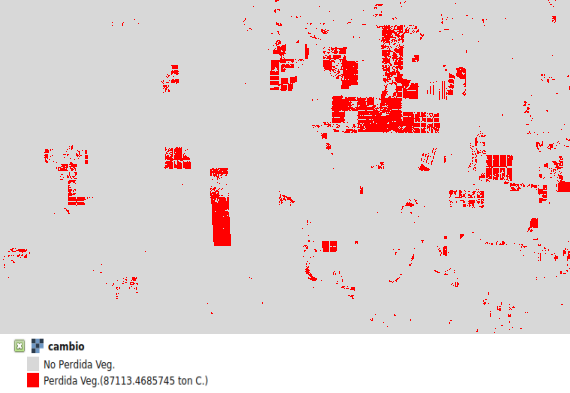
\includegraphics[width=0.8	\textwidth]{./Figures/cap4/resultadoMetodologia.png}
	\caption{Presentaci\'on del resultado. Mascara de perdida Forestal y la cantidad de carbono perdido.}
	\label{fig:resulPC}
\end{figure}
\subsection{Esquema general de la metodolog\'ia}
La metodolog\'ia presenta un esquema general descripta por el Algoritmo \ref{alg1}, desde los datos de entrada hasta su finalizaci\'on, de manera a brindar un resumen de los procesos realizados como también su aplicaci\'on en un ejemplo gr\'afico.
\begin{algorithm}
	\caption{Metodolog\'ia para estimar p\'erdida de carbono}
	\label{alg1}
	\begin{algorithmic}[1]
		\Require {$f_{t}(x,y,IRc);f_{t}(x,y,R), f_{t_{*}}(x,y,IRc);f_{t*}(x,y,R)$}
		\Statex
		\State $ I_{c_{fil \times col}}=  \begin{bmatrix}
		0 & \cdots & 0 \\
		\vdots & \ddots &  \vdots \\
		0 & \cdots & 0
		\end{bmatrix} $ \Comment{Indice de cambio $ I_{c} $}
		\State $ MC_{fil \times col} = \begin{bmatrix}
		1 & \cdots & 1 \\
		\vdots & \ddots &  \vdots \\
		1 & \cdots & 1
		\end{bmatrix} $ \Comment{Mascara de cambio $MC$}
		\State $ seguir = verdadero $ \Comment{Variable que controla la iterac\'on}
		\State $\mu_{anterior} =0$ \Comment{Media de $ I_{c} $ en la iteraci\'on anterior}
		\Statex
		\State $ iter = 0 $
		\While{$seguir$}
		
			\State \Comment{Se calculan las medias y desviaciones en funci\'on a una m\'ascara si no es la}
			\State \Comment{primera iteraci\'on (algoritmo \ref{alg:parametros})}
			\State $[\mu_{R,t},\mu_{IRc,t},\sigma_{R,t},\sigma_{IRc,t}] = \textsc{parametros}(f_{t}(x,y,R),f_{t}(x,y,IRc),MC)$		
			\State $[\mu_{R,t_{*}},\mu_{IRc,t_{*}},\sigma_{R,t_{*}},\sigma_{IRc,t_{*}}] = \textsc{parametros}(f_{t_{*}}(x,y,R),f_{t_{*}}(x,y,IRc),MC)$
			\Statex
			\State \Comment{Utilizar ecuaci\'on \ref{ec:normalizacion} para normalizar}
			\State $f_{t_{*}}^{Norm}(x,y,R) = \textsc{normalizar}(\mu_{R,t_{*}},\sigma_{R,t_{*}},\mu_{R,t},\sigma_{R,t},f_{t}(x,y,R),f_{t_{*}}(x,y,R))$  
			\State $f_{t_{*}}^{Norm}(x,y,IRc) = \textsc{normalizar}(\mu_{IRc,t_{*}},\sigma_{IRc,t_{*}},\mu_{IRc,t},\sigma_{IRc,t},f_{t}(x,y,IRc),f_{t_{*}}(x,y,IRc))$  
			
			\State \Comment{Utilizar ecuaci\'on \ref{e:ndvi} para el c\'alculo de NDVI}
			\State $ndvi_{f_{t}}=calcNDVI(f_{t}(x,y,R),f_{t}(x,y,IRc))$
			\State $ndvi_{f_{t_{*}}}=calcNDVI(f_{t}^{Norm}(x,y,R),f_{t}^{Norm}(x,y,IRc))$
			\Statex
			\State \Comment{Calculamos $ I_{c} $}
			\State $I_{c} = ndvi_{f_{t}} - ndvi_{f_{t_{*}}}$
			\State \Comment{Utilizar ecuaci\'on \ref{ec:continuar}}
			\State $seguir=\text{continuar}(\mu_{anterior},\textsc{media}(I_{c}))$
			\State $\mu_{anterior}=\textsc{media}(I_{c})$
			\Statex
			
%										\algstore{myalg}
%									\end{algorithmic}
%								\end{algorithm}
								
%								\begin{algorithm}                     
%									\begin{algorithmic} [1]                   % enter the algorithmic environment
%										\algrestore{myalg}
			\State \Comment{Calculamos $ MC $ seg\'un ecuaci\'on \ref{ec:umbMetodo}}
			\State $MC=\textsc{umbralizar}(I_{c})$	
			\Statex
			\State $iter++$
		\EndWhile	
		\Statex
		\State \Comment{Se determina la m\'ascara de vegetaci\'on seg\'un la secci\'on \ref{sec:discrForestalMet}}
		\State $MV=\textsc{mascaraVegetacion}(f_{t_{*}}^{Norm}(x,y,R),f_{t_{*}}^{Norm}(x,y,IRc),f_{t}(x,y,R),f_{t}(x,y,IRc))$
		\State 
		\State \Comment{Se determina la m\'ascara de perdida seg\'un la ecuaci\'on \ref{ec:umbMetodoMP}}
		\State $MP=\textsc{mascaraPerdida}(I_{c})$
		\Statex		
		\State \Comment{Se determina la m\'ascara de perdida forestal intersectando $ MC $ con $ MV $}
		\State $MPF=MP \textsc{ AND } MV $ 
		\Statex 		
		\State \Comment{Se estima la cantidad de carbono perdido mediante ecuaci\'on \ref{ec:carbonoFinalsumatoriam}}
		\State $CCP=sumatoria(MPF,I_{c})$
		\Statex 
		\Return $[CCP,MPF]$
		\Statex 
		
	\end{algorithmic}
\end{algorithm}

Dada una secuencia multitemporal ($ f_{t},f_{t_{*}} $), donde $ t<t_{*} $, con las bandas infrarroja cercana y roja de entrada $ (f_{t}(x,y,IRC)$, $f_{t}(x,y,R)$, $f_{t_{*}}(x,y,IRC)$,  $f_{t_{*}}(x,y,R)) $ de una peque\~{n}a porci\'on de cada imagen satelital, seg\'un la Figura \ref{fig:ejemplo_1}, se realiza un ejemplo con una porci\'on de $ 5 \times 5 $ para $ f_{t} $ y $ f_{t_{*}} $:
\begin{figure}[H]
	\centering
	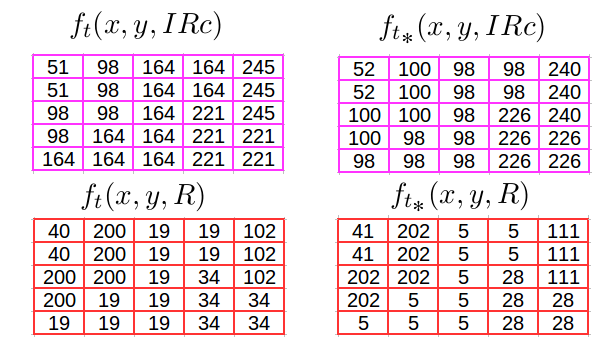
\includegraphics[width=0.8	\textwidth]{./Figures/cap4/ejemplo_entrada.png}
	\caption{Bandas de im\'agenes satelitales utilizados como entrada.}
	\label{fig:ejemplo_1}
\end{figure}
El proceso de iteraci\'on empieza normalizando radiom\'etricamente las bandas de $ f_{t_{*}} $ de manera a buscar la semejanza con las bandas de $ f_{t} $. La normalizaci\'on es realizado mediante la ecuaci\'on \ref{ec:normalizacion} habiendo calculado los par\'ametros estad\'isticos (Algoritmo \ref{alg:parametros}) en base a una mascara de cambio $ MC $, donde inicialmente sus niveles digitales valen $ 1 $. La Figura \ref{fig:ejemplo_2} nos muestra todos los procedimientos realizados en la primera iteraci\'on. 

\begin{figure}[H]
	\centering
	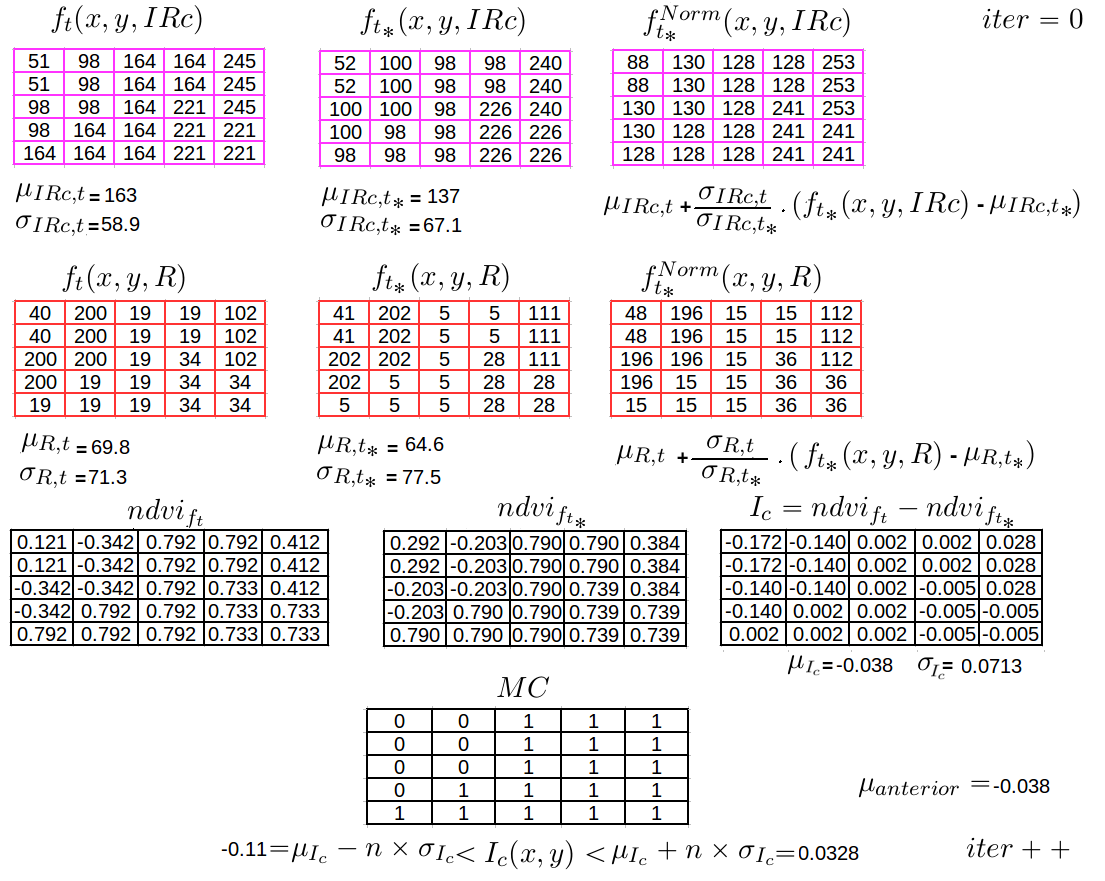
\includegraphics[width=1.0	\textwidth]{./Figures/cap4/ejemplo_iteracion_1.png}
	\caption{Primera iteraci\'on en el proceso de detecci\'on de cambio.}
	\label{fig:ejemplo_2}
\end{figure}
En la segunda iteraci\'on la mascara de cambio $ MC $ es tenido en cuenta para realizar el c\'alculo de los par\'ametros estad\'isticos solo sobre los pixeles que no sufrieron cambio ($ MC(x,y)=1 $). La Figura \ref{fig:ejemplo_3} nos muestra la segunda iteraci\'on, 
\begin{figure}[H]
	\centering
	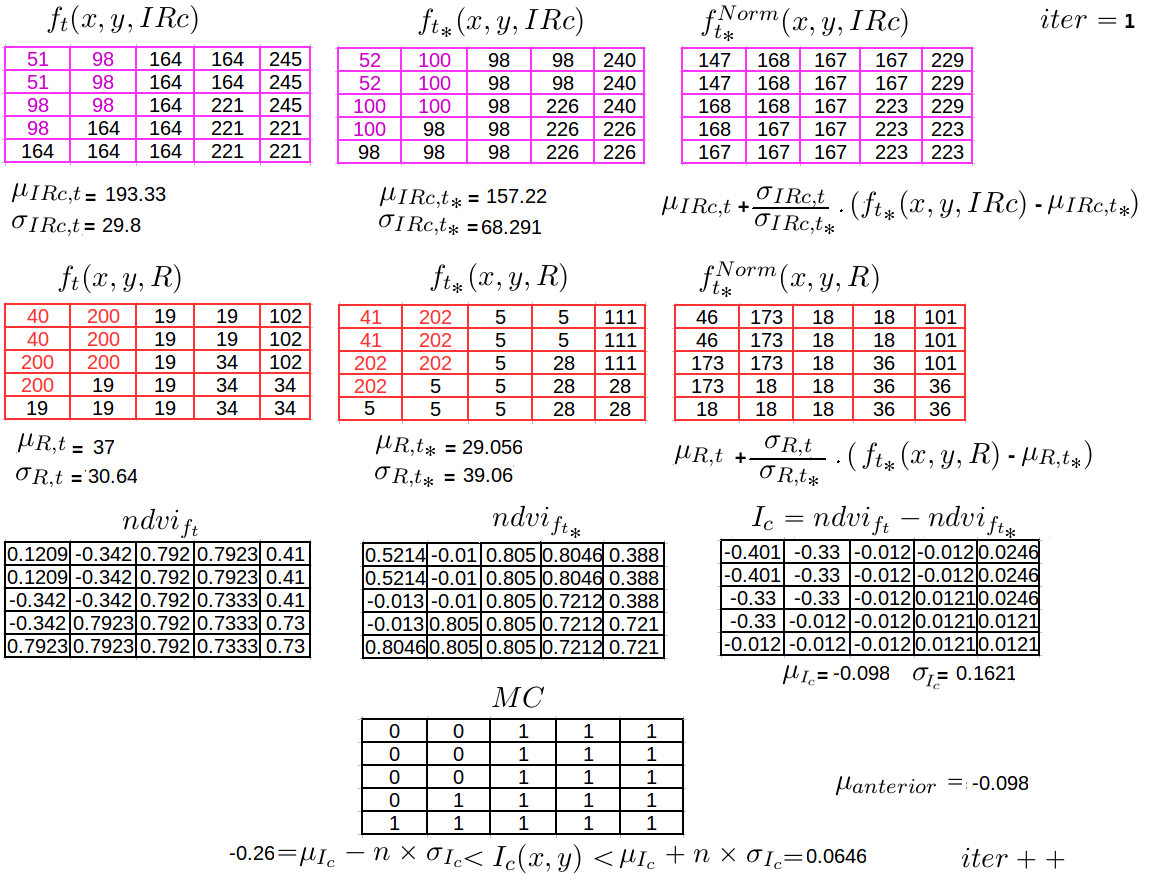
\includegraphics[width=1.0	\textwidth]{./Figures/cap4/ejemplo_iteracion_2.png}
	\caption{Segunda iteraci\'on en el proceso de detecci\'on de cambio.}
	\label{fig:ejemplo_3}
\end{figure}
En la Figura \ref{fig:ejemplo_4} podemos observar la siguiente iteraci\'on, donde la diferencia entre la media anterior $ \mu_{anterior} $ y la media de $ I_{c} $ actual ($ \mu_{I_{c}} $) cumple con la ecuaci\'on \ref{ec:continuar} para un $\epsilon=0 $, finalizando as\'i la iteraci\'on en la detecci\'on de cambio.
\begin{figure}[H]
	\centering
	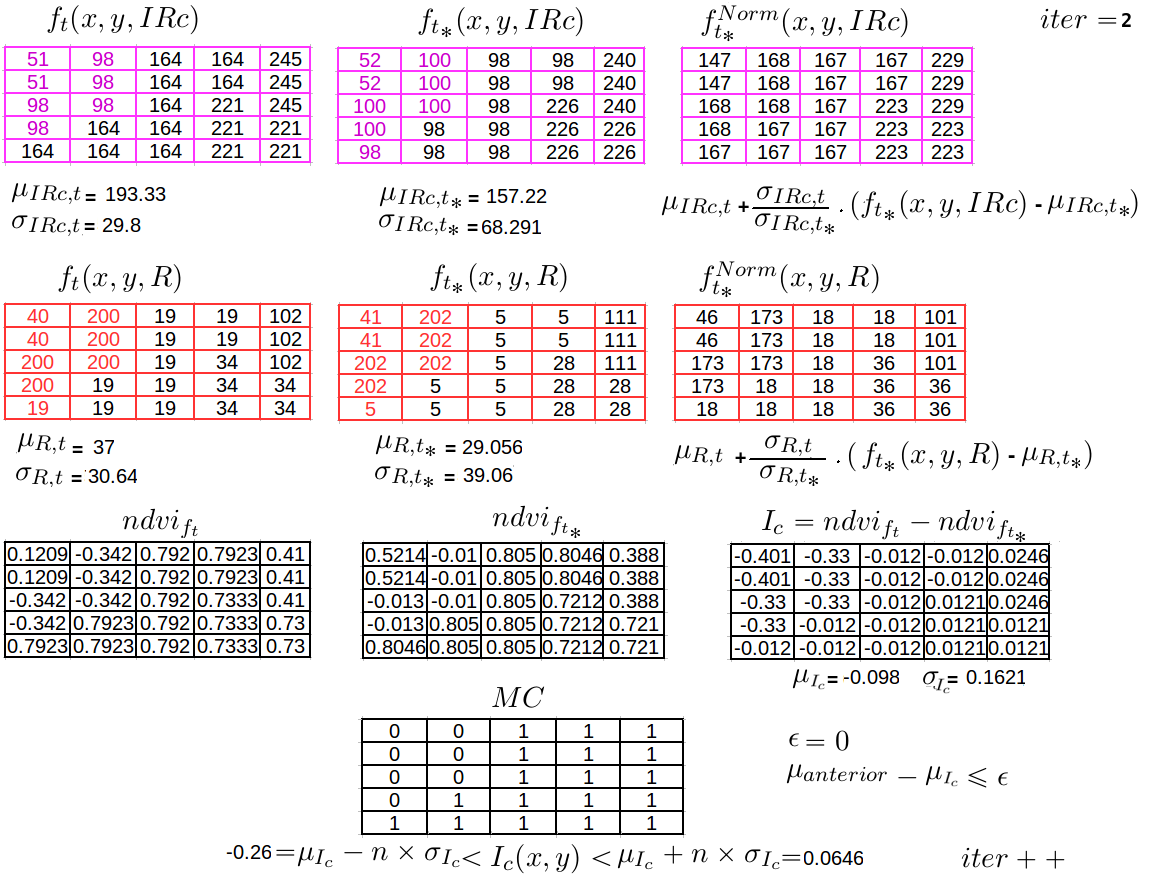
\includegraphics[width=1.0	\textwidth]{./Figures/cap4/ejemplo_iteracion_3.png}
	\caption{\'Ultima iteraci\'on en el proceso de detecci\'on de cambio.}
	\label{fig:ejemplo_4}
\end{figure}
La Figura \ref{fig:ejemplo_5} nos muestra como es obtenida la mascara de vegetaci\'on $ MV $ en en funci\'on a $ ndvi_{f_{t}} $ y $ ndvi_{f_{t_{*}}} $
\begin{figure}[H]
	\centering
	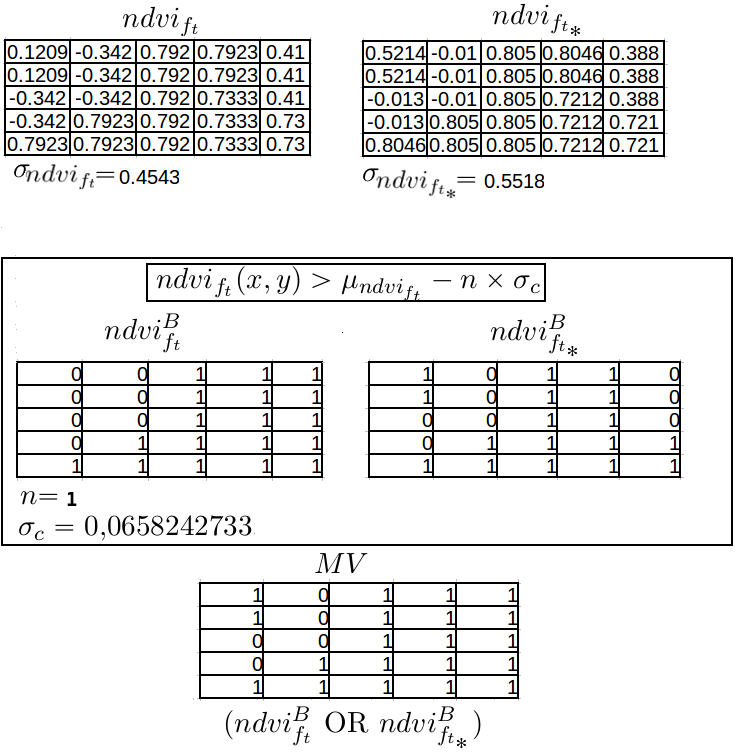
\includegraphics[width=0.8	\textwidth]{./Figures/cap4/ejemplo_ndvi.png}
	\caption{Determinaci\'on de la m\'ascara de vegetaci\'on $ MV $.}
	\label{fig:ejemplo_5}
\end{figure}
La Figura \ref{fig:ejemplo_6} podemos observar la forma en que es calculado la m\'ascara de perdida forestal y su cuantificaci\'on. En la figura se resalta en un cuadro rojo el resultado esperado por la metodología. 
\begin{figure}[H]
	\centering
	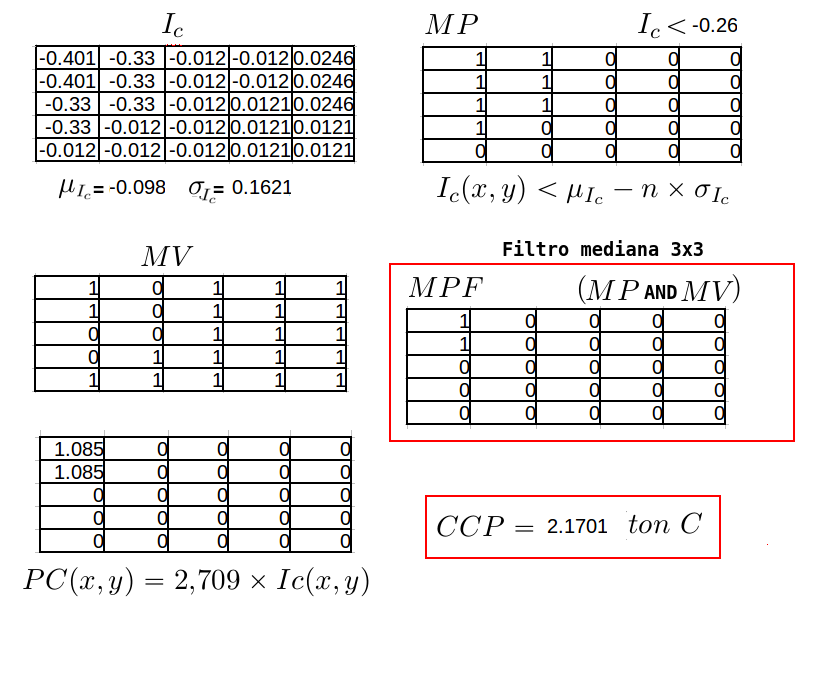
\includegraphics[width=0.8	\textwidth]{./Figures/cap4/ejemplo_resultado.png}
	\caption{Mascara de cambio forestal y cuantificaci\'on de perdida de carbono forestal.}
	\label{fig:ejemplo_6}
\end{figure}
\section{Resumen}
En este capitulo se describen los materiales y los tres procedimientos generales que componen la metodolog\'ia propuesta. La im\'agenes infrarroja cercana y roja de las dos fechas inicialmente deben pasar por un proceso de correcci\'on de errores del sensor y de ubicaci\'on geogr\'afica para realizar el an\'alisis multitemporal en la detecci\'on de cambio forestal. Una vez detectado la perdida forestal entre las fechas del proceso de detecci\'on de cambio, se realiza la estimaci\'on de carbono en base a una ecuaci\'on de regresi\'on hallado por un estudio previo. El resultado consiste en un mapa de perdida forestal junto a la cuantificaci\'on en toneladas de carbono perdidos.